\documentclass[portrait,final]{baposter}

\tracingstats=2

\usepackage{times}
\usepackage{calc}
\usepackage{graphicx}
\usepackage{amsmath}
\usepackage{amssymb}
\usepackage{relsize}
\usepackage{multirow}
\usepackage{bm}

\usepackage{graphicx}
\usepackage{multicol}
\usepackage{wrapfig}

\usepackage{pgfbaselayers}
\pgfdeclarelayer{background}
\pgfdeclarelayer{foreground}
\pgfsetlayers{background,main,foreground}

\usepackage{helvet}
%\usepackage{bookman}
\usepackage{palatino}

\newcommand{\captionfont}{\footnotesize}

\selectcolormodel{rgb}

\graphicspath{{images/}}

%%%%%%%%%%%%%%%%%%%%%%%%%%%%%%%%%%%%%%%%%%%%%%%%%%%%%%%%%%%%%%%%%%%%%%%%%%%%%%%%
%%%% Some math symbols used in the text
%%%%%%%%%%%%%%%%%%%%%%%%%%%%%%%%%%%%%%%%%%%%%%%%%%%%%%%%%%%%%%%%%%%%%%%%%%%%%%%%
% Format 
\newcommand{\Matrix}[1]{\begin{bmatrix} #1 \end{bmatrix}}
\newcommand{\Vector}[1]{\Matrix{#1}}
\newcommand*{\SET}[1]  {\ensuremath{\mathcal{#1}}}
\newcommand*{\MAT}[1]  {\ensuremath{\mathbf{#1}}}
\newcommand*{\VEC}[1]  {\ensuremath{\bm{#1}}}
\newcommand*{\CONST}[1]{\ensuremath{\mathit{#1}}}
\newcommand*{\norm}[1]{\mathopen\| #1 \mathclose\|}% use instead of $\|x\|$
\newcommand*{\abs}[1]{\mathopen| #1 \mathclose|}% use instead of $\|x\|$
\newcommand*{\absLR}[1]{\left| #1 \right|}% use instead of $\|x\|$

\def\norm#1{\mathopen\| #1 \mathclose\|}% use instead of $\|x\|$
\newcommand{\normLR}[1]{\left\| #1 \right\|}% use instead of $\|x\|$

%%%%%%%%%%%%%%%%%%%%%%%%%%%%%%%%%%%%%%%%%%%%%%%%%%%%%%%%%%%%%%%%%%%%%%%%%%%%%%%%
% Multicol Settings
%%%%%%%%%%%%%%%%%%%%%%%%%%%%%%%%%%%%%%%%%%%%%%%%%%%%%%%%%%%%%%%%%%%%%%%%%%%%%%%%
\setlength{\columnsep}{0.7em}
\setlength{\columnseprule}{0mm}


%%%%%%%%%%%%%%%%%%%%%%%%%%%%%%%%%%%%%%%%%%%%%%%%%%%%%%%%%%%%%%%%%%%%%%%%%%%%%%%%
% Save space in lists. Use this after the opening of the list
%%%%%%%%%%%%%%%%%%%%%%%%%%%%%%%%%%%%%%%%%%%%%%%%%%%%%%%%%%%%%%%%%%%%%%%%%%%%%%%%
\newcommand{\compresslist}{%
\setlength{\itemsep}{1pt}%
\setlength{\parskip}{0pt}%
\setlength{\parsep}{0pt}%
}


%%%%%%%%%%%%%%%%%%%%%%%%%%%%%%%%%%%%%%%%%%%%%%%%%%%%%%%%%%%%%%%%%%%%%%%%%%%%%%
%%% Begin of Document
%%%%%%%%%%%%%%%%%%%%%%%%%%%%%%%%%%%%%%%%%%%%%%%%%%%%%%%%%%%%%%%%%%%%%%%%%%%%%%

\begin{document}

%%%%%%%%%%%%%%%%%%%%%%%%%%%%%%%%%%%%%%%%%%%%%%%%%%%%%%%%%%%%%%%%%%%%%%%%%%%%%%
%%% Here starts the poster
%%%---------------------------------------------------------------------------
%%% Format it to your taste with the options
%%%%%%%%%%%%%%%%%%%%%%%%%%%%%%%%%%%%%%%%%%%%%%%%%%%%%%%%%%%%%%%%%%%%%%%%%%%%%%
% Define some colors
%\definecolor{silver}{cmyk}{0,0,0,0.3}
%\definecolor{yellow}{cmyk}{0,0,0.9,0.0}
%\definecolor{reddishyellow}{cmyk}{0,0.22,1.0,0.0}
%\definecolor{black}{cmyk}{0,0,0.0,1.0}
%\definecolor{darkYellow}{cmyk}{0,0,1.0,0.5}
%\definecolor{darkSilver}{cmyk}{0,0,0,0.1}

%\definecolor{lightyellow}{cmyk}{0,0,0.3,0.0}
%\definecolor{lighteryellow}{cmyk}{0,0,0.1,0.0}
%\definecolor{lighteryellow}{cmyk}{0,0,0.1,0.0}
%\definecolor{lightestyellow}{cmyk}{0,0,0.05,0.0}

\definecolor{black}{rgb}{0,0,0}
\definecolor{white}{rgb}{255,255,255}

% SU_blue
% \definecolor{SU_blue}{rgb}{0.000000,0.184314,0.372549}
\definecolor{SU_blue}{rgb}{0.098039, 0.329411,0.729411}
\definecolor{SU_blue80}{rgb}{0.000000,0.147451,0.298039}
\definecolor{SU_blue60}{rgb}{0.000000,0.110588,0.223529}
\definecolor{SU_blue40}{rgb}{0.000000,0.073725,0.149020}
\definecolor{SU_blue20}{rgb}{0.000000,0.036863,0.074510}
% SU_olive
\definecolor{SU_olive}{rgb}{0.639216,0.658824,0.419608}
\definecolor{SU_olive80}{rgb}{0.511373,0.527059,0.335686}
\definecolor{SU_olive60}{rgb}{0.383529,0.395294,0.251765}
\definecolor{SU_olive40}{rgb}{0.255686,0.263529,0.167843}
\definecolor{SU_olive20}{rgb}{0.127843,0.131765,0.083922}
% SU_sky
\definecolor{SU_sky}{rgb}{0.674510,0.870588,0.901961}
\definecolor{SU_sky80}{rgb}{0.539608,0.696471,0.721569}
\definecolor{SU_sky60}{rgb}{0.404706,0.522353,0.541176}
\definecolor{SU_sky40}{rgb}{0.269804,0.348235,0.360784}
\definecolor{SU_sky20}{rgb}{0.134902,0.174118,0.180392}
% SU_water
\definecolor{SU_water}{rgb}{0.607843,0.698039,0.807843}
\definecolor{SU_water80}{rgb}{0.486275,0.558431,0.646275}
\definecolor{SU_water60}{rgb}{0.364706,0.418824,0.484706}
\definecolor{SU_water40}{rgb}{0.243137,0.279216,0.323137}
\definecolor{SU_water20}{rgb}{0.121569,0.139608,0.161569}
% SU_fire
\definecolor{SU_fire}{rgb}{0.850980,0.368627,0.000000}
\definecolor{SU_fire80}{rgb}{0.680784,0.294902,0.000000}
\definecolor{SU_fire60}{rgb}{0.510588,0.221176,0.000000}
\definecolor{SU_fire40}{rgb}{0.340392,0.147451,0.000000}
\definecolor{SU_fire20}{rgb}{0.170196,0.073725,0.000000}
% SU_silver
\definecolor{SU_silver}{rgb}{0.737255,0.741176,0.737255}
\definecolor{SU_silver80}{rgb}{0.589804,0.592941,0.589804}
\definecolor{SU_silver60}{rgb}{0.442353,0.444706,0.442353}
\definecolor{SU_silver40}{rgb}{0.294902,0.296471,0.294902}
\definecolor{SU_silver20}{rgb}{0.147451,0.148235,0.147451}


%%
\typeout{Poster Starts}
\background{
  \begin{tikzpicture}[remember picture,overlay]%
    \draw (current page.north west)+(-2em,2em) node[anchor=north west] {\includegraphics[height=1.1\textheight]{silhouettes_background}};
  \end{tikzpicture}%
}

\newlength{\leftimgwidth}
\begin{poster}%
  % Poster Options
  {
  % Show grid to help with alignment
  grid=no,
  % Column spacing
  colspacing=1em,
  % Color style
  bgColorOne=white,
  bgColorTwo=SU_blue,
  borderColor=white,
  headerColorOne=SU_blue,
  headerColorTwo=SU_blue,
  headerFontColor=white,
  boxColorOne=white, %SU_sky,
  boxColorTwo=SU_sky,
  % Format of textbox
  textborder=roundedleft,
  % Format of text header
  eyecatcher=yes,
  headerborder=open,
  headerheight=0.08\textheight,
  headershape=roundedright,
  headershade=plain,
  headerfont=\Large\textsf, %Sans Serif
  boxshade=plain,
%  background=shade-tb,
  background=plain,
  linewidth=2pt
  }
  % Eye Catcher
  {
\includegraphics[height=7em]{Kth_logo.png}} % No eye catcher for this poster. (eyecatcher=no above). If an eye catcher is present, the title is centered between eye-catcher and logo.
  % Title
  {\sf %Sans Serif
  %\bf% Serif
  \color{black} Sequence learning with the BCPNN rule}
  % Authors
  {\sf %Sans Serif
  % Serif
  \vspace{0.5em}
  \color{SU_fire} Ram\'on Mart\'inez,  Anders Lansner, Pawel Herman
  }
  % University logo
  {% The makebox allows the title to flow into the logo, this is a hack because of the L shaped logo.
    \makebox[8em][r]{%
      \begin{minipage}{16em}
        \hfill
        %\includegraphics[height=7.0em]{CERN_logo_white_on_transparent}
        \vspace{-10pt}
        
\includegraphics[height=7.0em]{euro_spin_logo.jpg}
      \end{minipage}
    }
  }

  \tikzstyle{light shaded}=[top color=baposterBGtwo!30!white,bottom color=baposterBGone!30!white,shading=axis,shading angle=30]

  % Width of left inset image
     \setlength{\leftimgwidth}{0.78em+8.0em}

%%%%%%%%%%%%%%%%%%%%%%%%%%%%%%%%%%%%%%%%%%%%%%%%%%%%%%%%%%%%%%%%%%%%%%%%%%%%%%
%%% Now define the boxes that make up the poster
%%%---------------------------------------------------------------------------
%%% Each box has a name and can be placed absolutely or relatively.
%%% The only inconvenience is that you can only specify a relative position 
%%% towards an already declared box. So if you have a box attached to the 
%%% bottom, one to the top and a third one which should be in between, you 
%%% have to specify the top and bottom boxes before you specify the middle 
%%% box.
%%%%%%%%%%%%%%%%%%%%%%%%%%%%%%%%%%%%%%%%%%%%%%%%%%%%%%%%%%%%%%%%%%%%%%%%%%%%%%
    %
    % A colored circle useful as a bullet with an adjustably strong filling
    \newcommand{\coloredcircle}[1]{%
      \tikz{\useasboundingbox (-0.2em,-0.32em) rectangle(0.2em,0.32em); \draw[draw=black,fill=SU_blue!80!black!#1!white,line width=0.03em] (0,0) circle(0.18em);}}

%%%%%%%%%%%%%%%%%%%%%%%%%%%%%%%%%%%%%%%%%%%%%%%%%%%%%%%%%%%%%%%%%%%%%%%%%%%%%%
  \headerbox{Sequence Learning}{name=sequences,column=0,row=0}{
%%%%%%%%%%%%%%%%%%%%%%%%%%%%%%%%%%%%%%%%%%%%%%%%%%%%%%%%%%%%%%%%%%%%%%%%%%%%%%
  {}
How can neocortical microcircuits encode sequences of activity? How can a stable sequential dynamics self-organize withing the bounds of the biological constrains? As early as 1950 Karl Lashley \cite{lashley} advocated that the ability to sequence actions is the essential cognitive ability of human, how can we account for it? Since then we have found sequential population bursts in the activity related to the following behaviors:

\begin{itemize}
\item Motor
\item Sensory
\item Memory
\item Decision Making
\end{itemize}

Here we propose a generic model that is a step ahead in solving the riddles above.
}

%%%%%%%%%%%%%%%%%%%%%%%%%%%%%%%%%%%%%%%%%%%%%%%%%%%%%%%%%%%%%%%%%%%%%%%%%%%%%%
  \headerbox{NMDA Connectivity Matrix}{name=connectivity,column=0,span=1,below=sequences}{
%%%%%%%%%%%%%%%%%%%%%%%%%%%%%%%%%%%%%%%%%%%%%%%%%%%%%%%%%%%%%%%%%%%%%%%%%%%%%%
Here we show different arragnments of the connectivity matrix for different training schemes:

\begin{enumerate}
\item Simple sequence.
\item Sequences with overlap.
\item Sequences with overload.
\end{enumerate}
	
	\begin{center}
    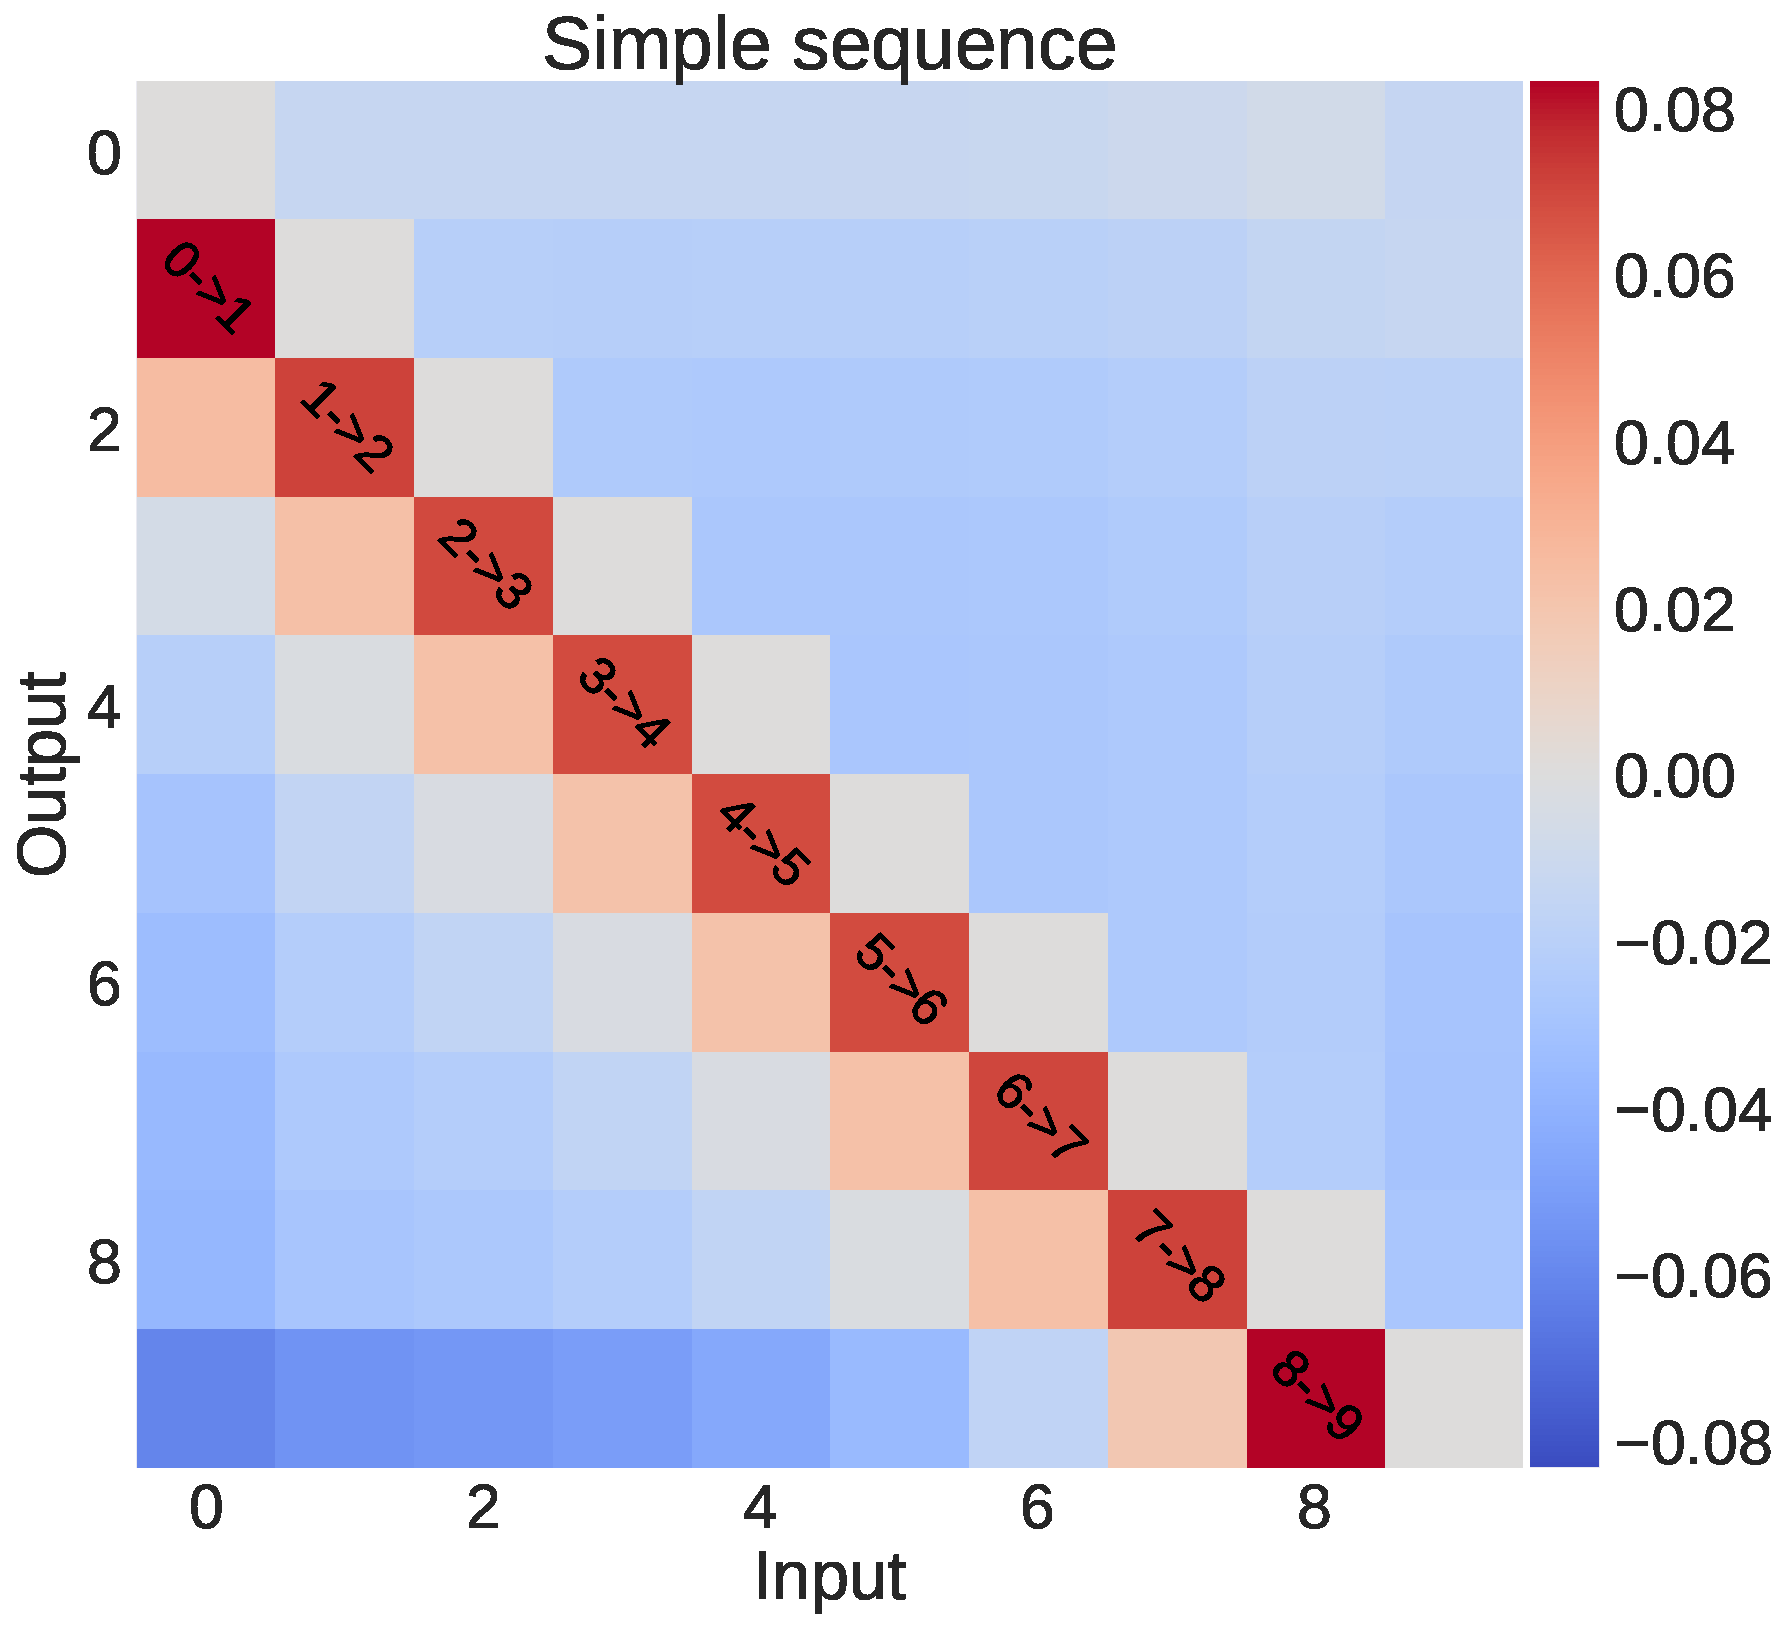
\includegraphics[scale=0.14]{matrix_normal.pdf}
  	\end{center}
  
  
  \begin{center}
    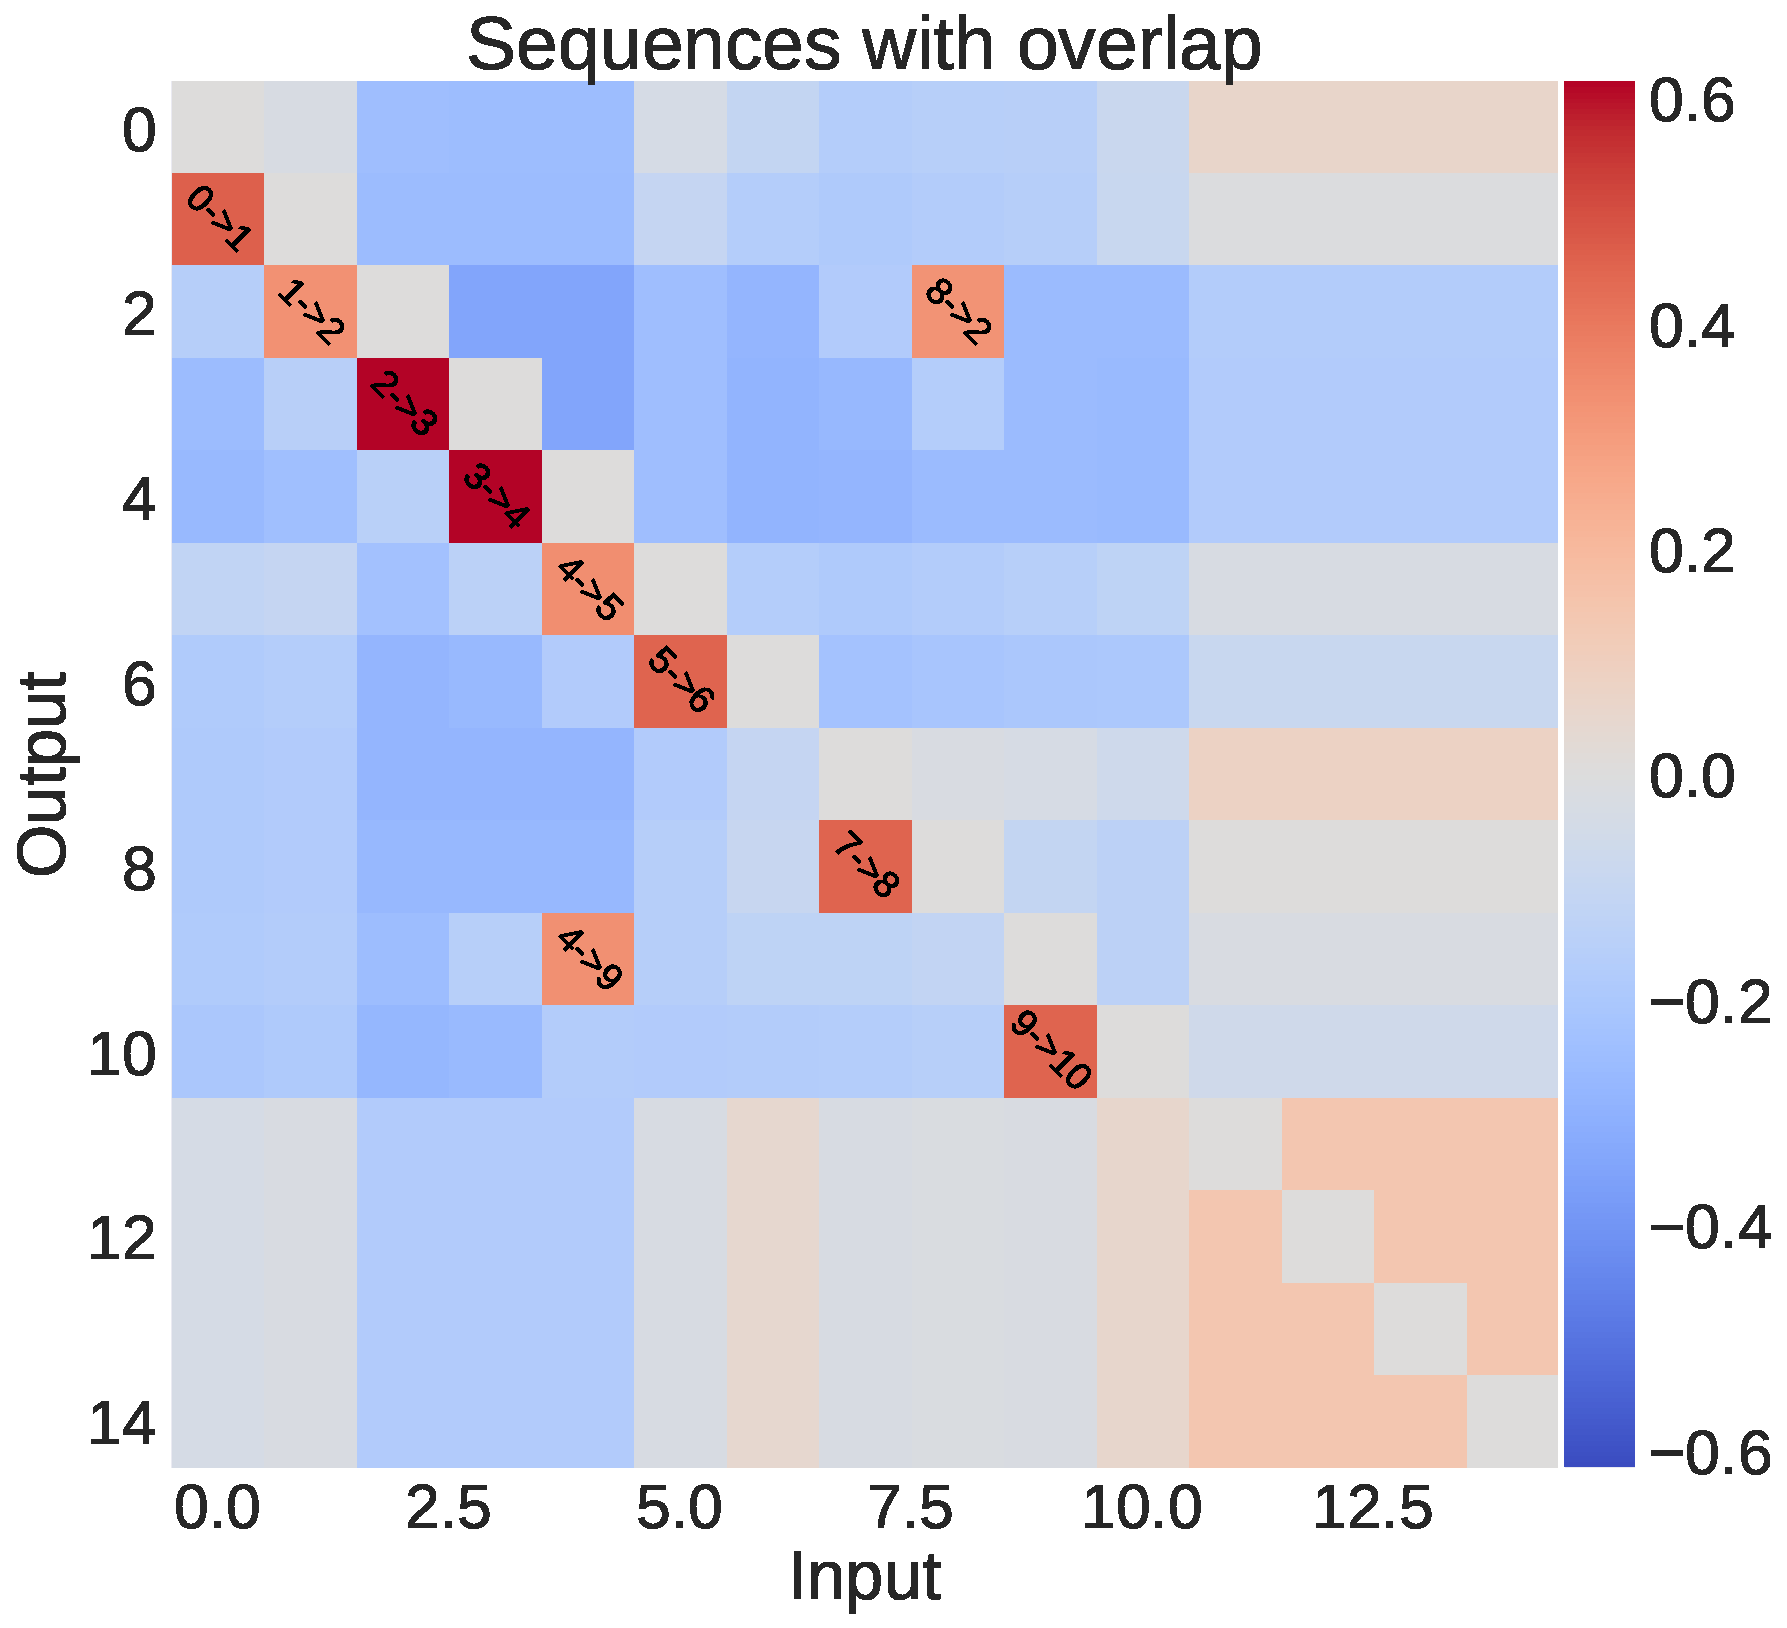
\includegraphics[scale=0.14]{matrix_overlap.pdf}
  	\end{center}
  	
  	\begin{center}
    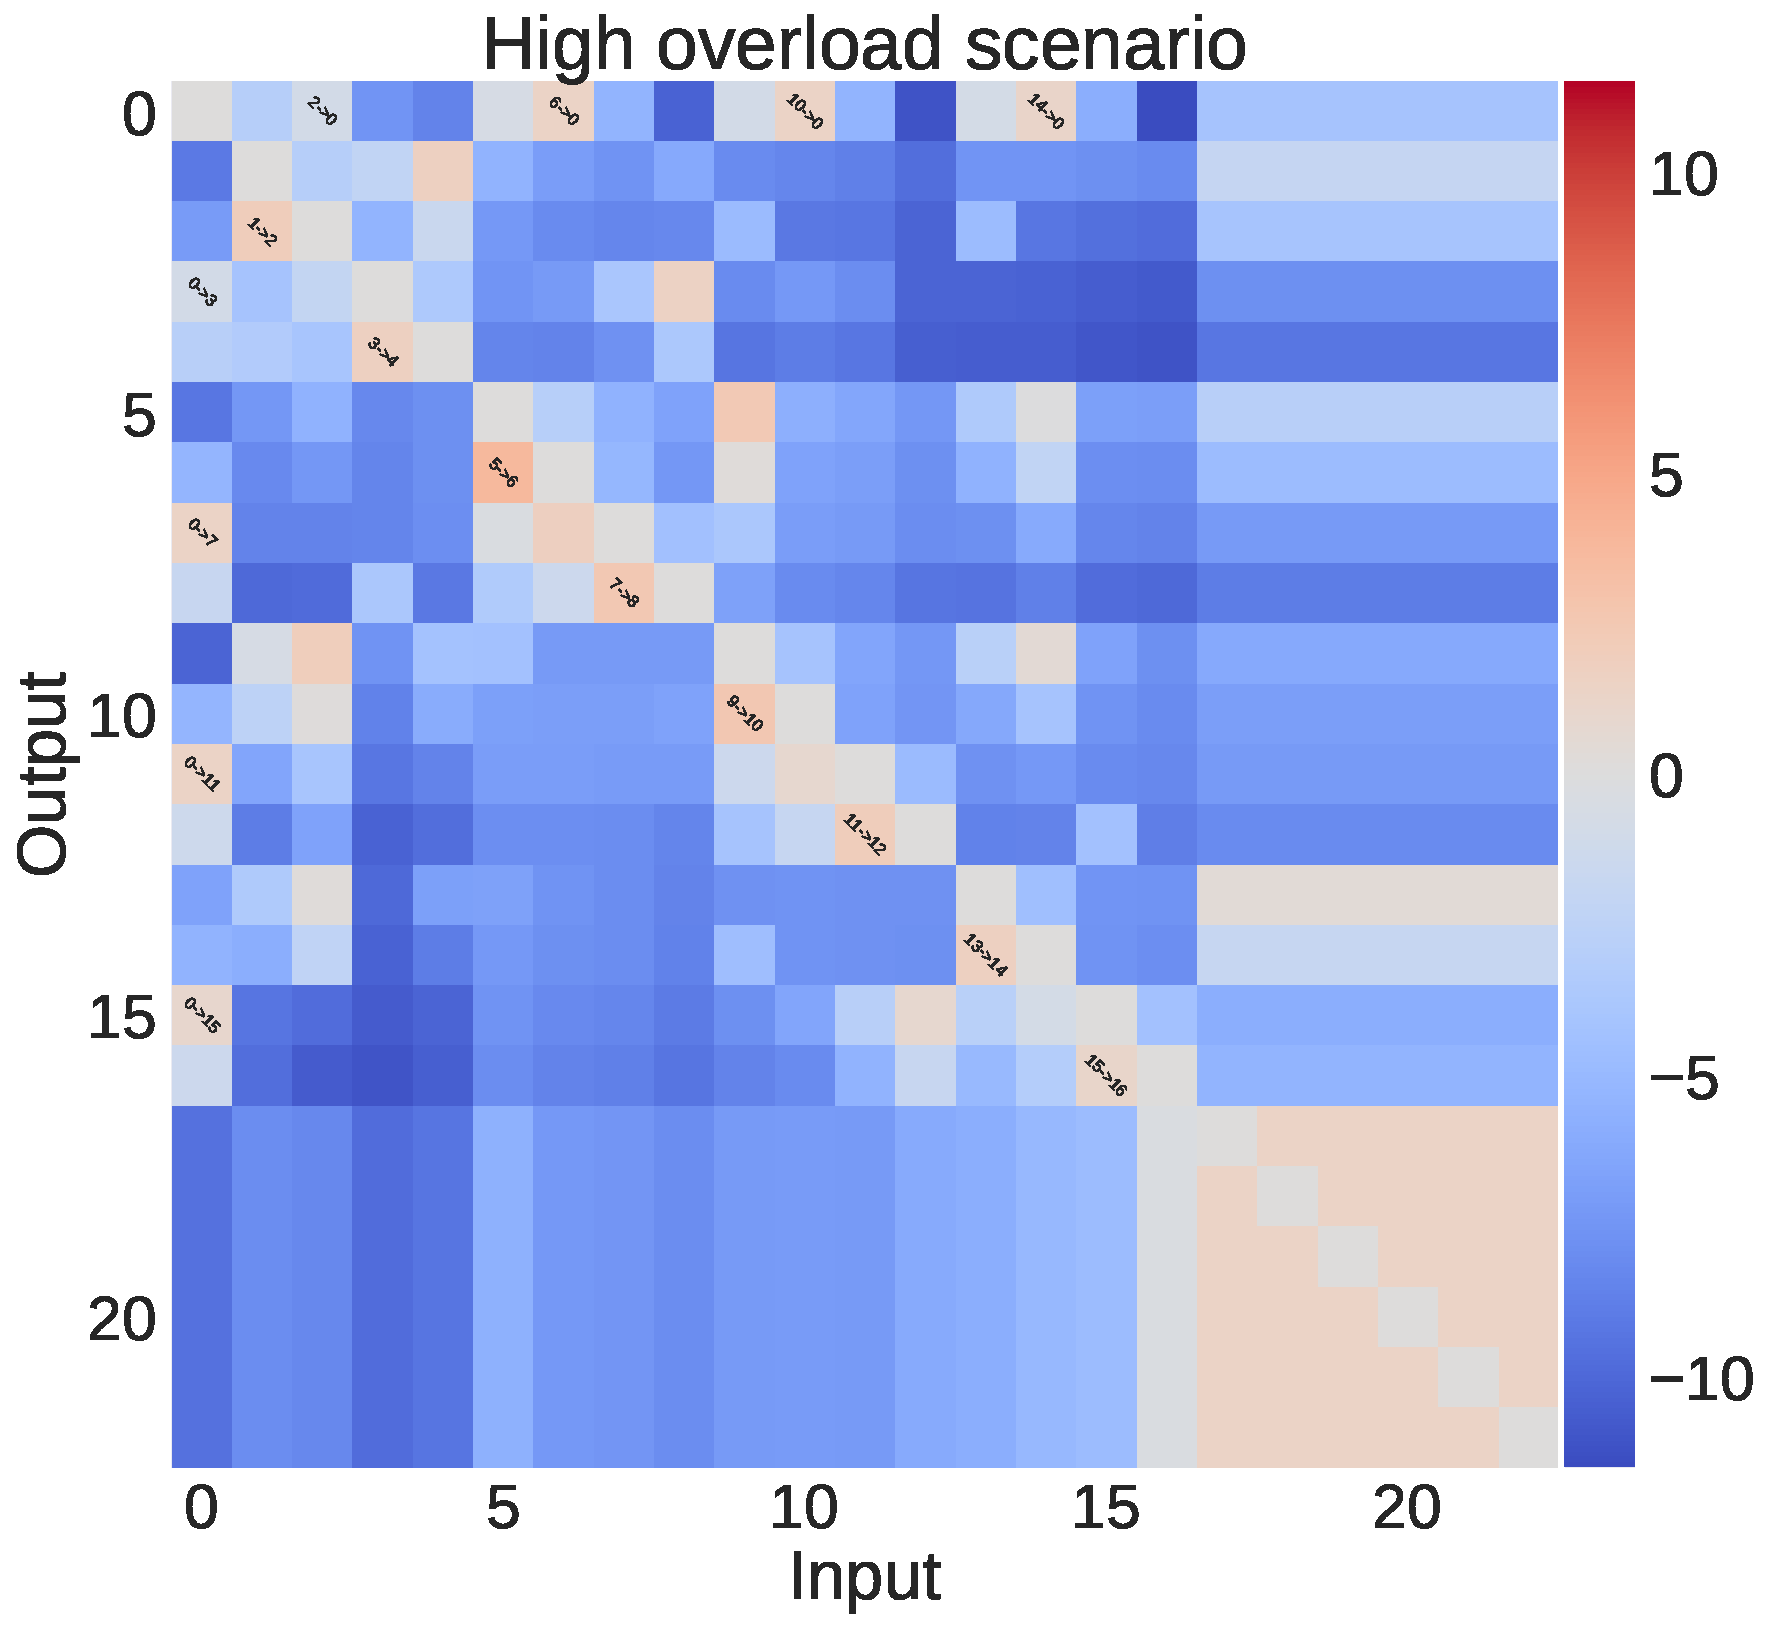
\includegraphics[scale=0.14]{matrix_overload.pdf}
  	\end{center}
}



%%%%%%%%%%%%%%%%%%%%%%%%%%%%%%%%%%%%%%%%%%%%%%%%%%%%%%%%%%%%%%%%%%%%%%%%%%%%%%
  \headerbox{References}{name=references,column=0,above=bottom} {
%%%%%%%%%%%%%%%%%%%%%%%%%%%%%%%%%%%%%%%%%%%%%%%%%%%%%%%%%%%%%%%%%%%%%%%%%%%%%%
    \smaller
    \vspace{-0.4em}
    \bibliographystyle{ieee}
    \renewcommand{\section}[2]{\vskip 0.05em}
      \begin{thebibliography}{1}\itemsep=-0.01em
      \setlength{\baselineskip}{0.4em}
      
      \bibitem{phil}
       Tully, Philip J., Henrik Lind\'en, Matthias H. Hennig, and Anders Lansner. 
		\newblock{e1004954.}
        \newblock {\em PLoS Comput Biol 12, no. 5 (2016)}
      \bibitem{sandberg}
      \vspace{5pt}
        Sandberg, Anders, Anders Lansner, Karl Magnus Petersson, and Ekeberg
		\newblock{371(1):179-194}
        \newblock {\em Network: Computation in neural systems 13, no. 2 (2002))}
      \bibitem{lashley}
      \vspace{5pt}
         Lashley, Karl Spencer
		\newblock{pp. 112-136}
        \newblock {\em Cerebral mechanisms in behavior. 1951}
      \end{thebibliography} 
  }


%%%%%%%%%%%%%%%%%%%%%%%%%%%%%%%%%%%%%%%%%%%%%%%%%%%%%%%%%%%%%%%%%%%%%%%%%%%%%%
  \headerbox{The Model}{name=model,column=1,span=2}{
%%%%%%%%%%%%%%%%%%%%%%%%%%%%%%%%%%%%%%%%%%%%%%%%%%%%%%%%%%%%%%%%%%%%%%%%%%%%%%
\begin{multicols}{2}

\begin{itemize}
\item Previous work has shown that the BCPNN rule can learn sequences in a spike based attractor model with modular structure \cite{phil}.
\item Using the firing-rate version of the model \cite{sandberg} with both fast (AMPA) and slow (NMDA) connectivity we study the capabilities of the system for pattern and sequence storage. \cite{sandberg}.
\end{itemize}

\begin{align*}
\tau_m \dfrac{s_i}{dt} &= \beta_i + \sum_{j} w_{ij} o_j + a_i - s_i \\
o &= \frac{exp(s_i)}{\sum_j exp(s_j)} \\
\tau_z \dfrac{dz_i}{dt} &= o_{i, k} - z_{i} \\
\tau_p \dfrac{dp_i}{dt} &= z_i(t) - p_i(t)  \\  
\tau_p \dfrac{dp_{ij}}{dt} &= z_i(t) z_j(t) - p_{ij}(t)\\
w_{ij} &= \log(\frac{p_{ij}}{p_i p_j}) \\
\beta_i &= \log(p_i) 
\end{align*}

Due to a local transition rule in absence of noise this model can recall a sequence of arbitrary length. Moreover, it can perform within certain limitations both \textbf{sequence completion} and \textbf{sequence disambiguation}. 
  \begin{center}
    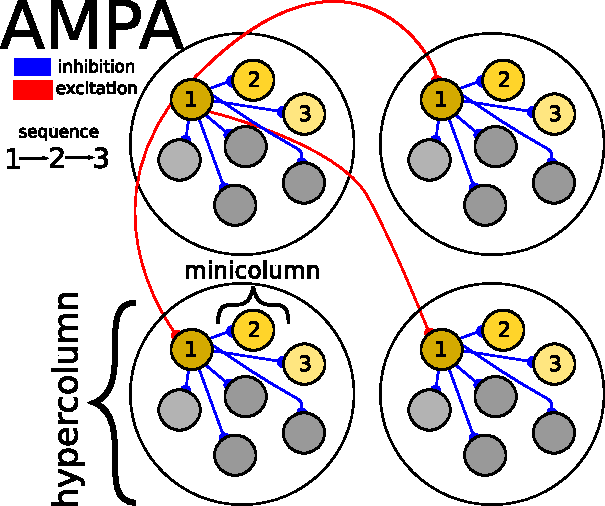
\includegraphics[scale=0.6]{ampa2.pdf}
 \end{center}
 
 \begin{center}
	\smaller Note that in both diagrams we only show the connections emanating from the first minicolumn in the top-left hypercolumn. 
	\end{center}
  
  \begin{center}
    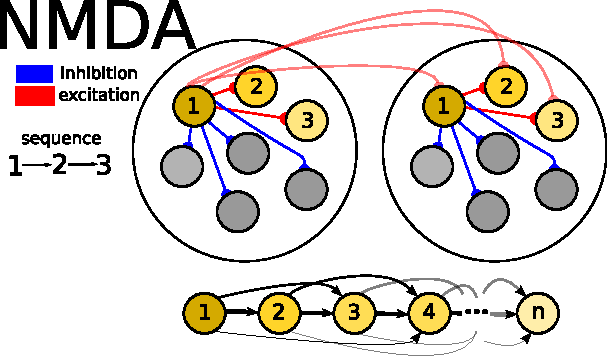
\includegraphics[scale=0.6]{nmda4.pdf}
  \end{center}
  
\end{multicols}

  }

%%%%%%%%%%%%%%%%%%%%%%%%%%%%%%%%%%%%%%%%%%%%%%%%%%%%%%%%%%%%%%%%%%%%%%%%%%%%%%
  \headerbox{Chains}{name=chains,column=1,span=2, below=model}{
%%%%%%%%%%%%%%%%%%%%%%%%%%%%%%%%%%%%%%%%%%%%%%%%%%%%%%%%%%%%%%%%%%%%%%%%%%%%%%
\vspace{1em}
\begin{multicols}{2}

\begin{itemize}
\item We stored more complicated sequences in order to probe how effective is our system at retrieving them.
\item Two relevant parameters to parametrize the space of all the possible sequences are \textbf{overlap} and \textbf{overload}. 
\end{itemize}

\begin{center}
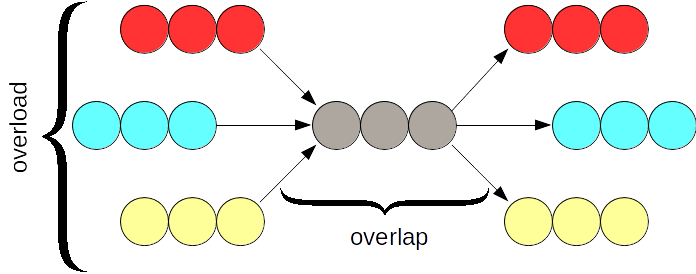
\includegraphics[scale=0.30]{scheme.png}
\end{center}

\end{multicols}

}

%%%%%%%%%%%%%%%%%%%%%%%%%%%%%%%%%%%%%%%%%%%%%%%%%%%%%%%%%%%%%%%%%%%%%%%%%%%%%%%
\headerbox{Overlap}{name=tau, column=1,span=1, below=chains}{
%%%%%%%%%%%%%%%%%%%%%%%%%%%%%%%%%%%%%%%%%%%%%%%%%%%%%%%%%%%%%%%%%%%%%%%%%%%%%%%


We calculate whether our system is able to correctly process the sequence with some overlap for different values of the parameter $\tau_z$ of the NMDA. 
\begin{center}
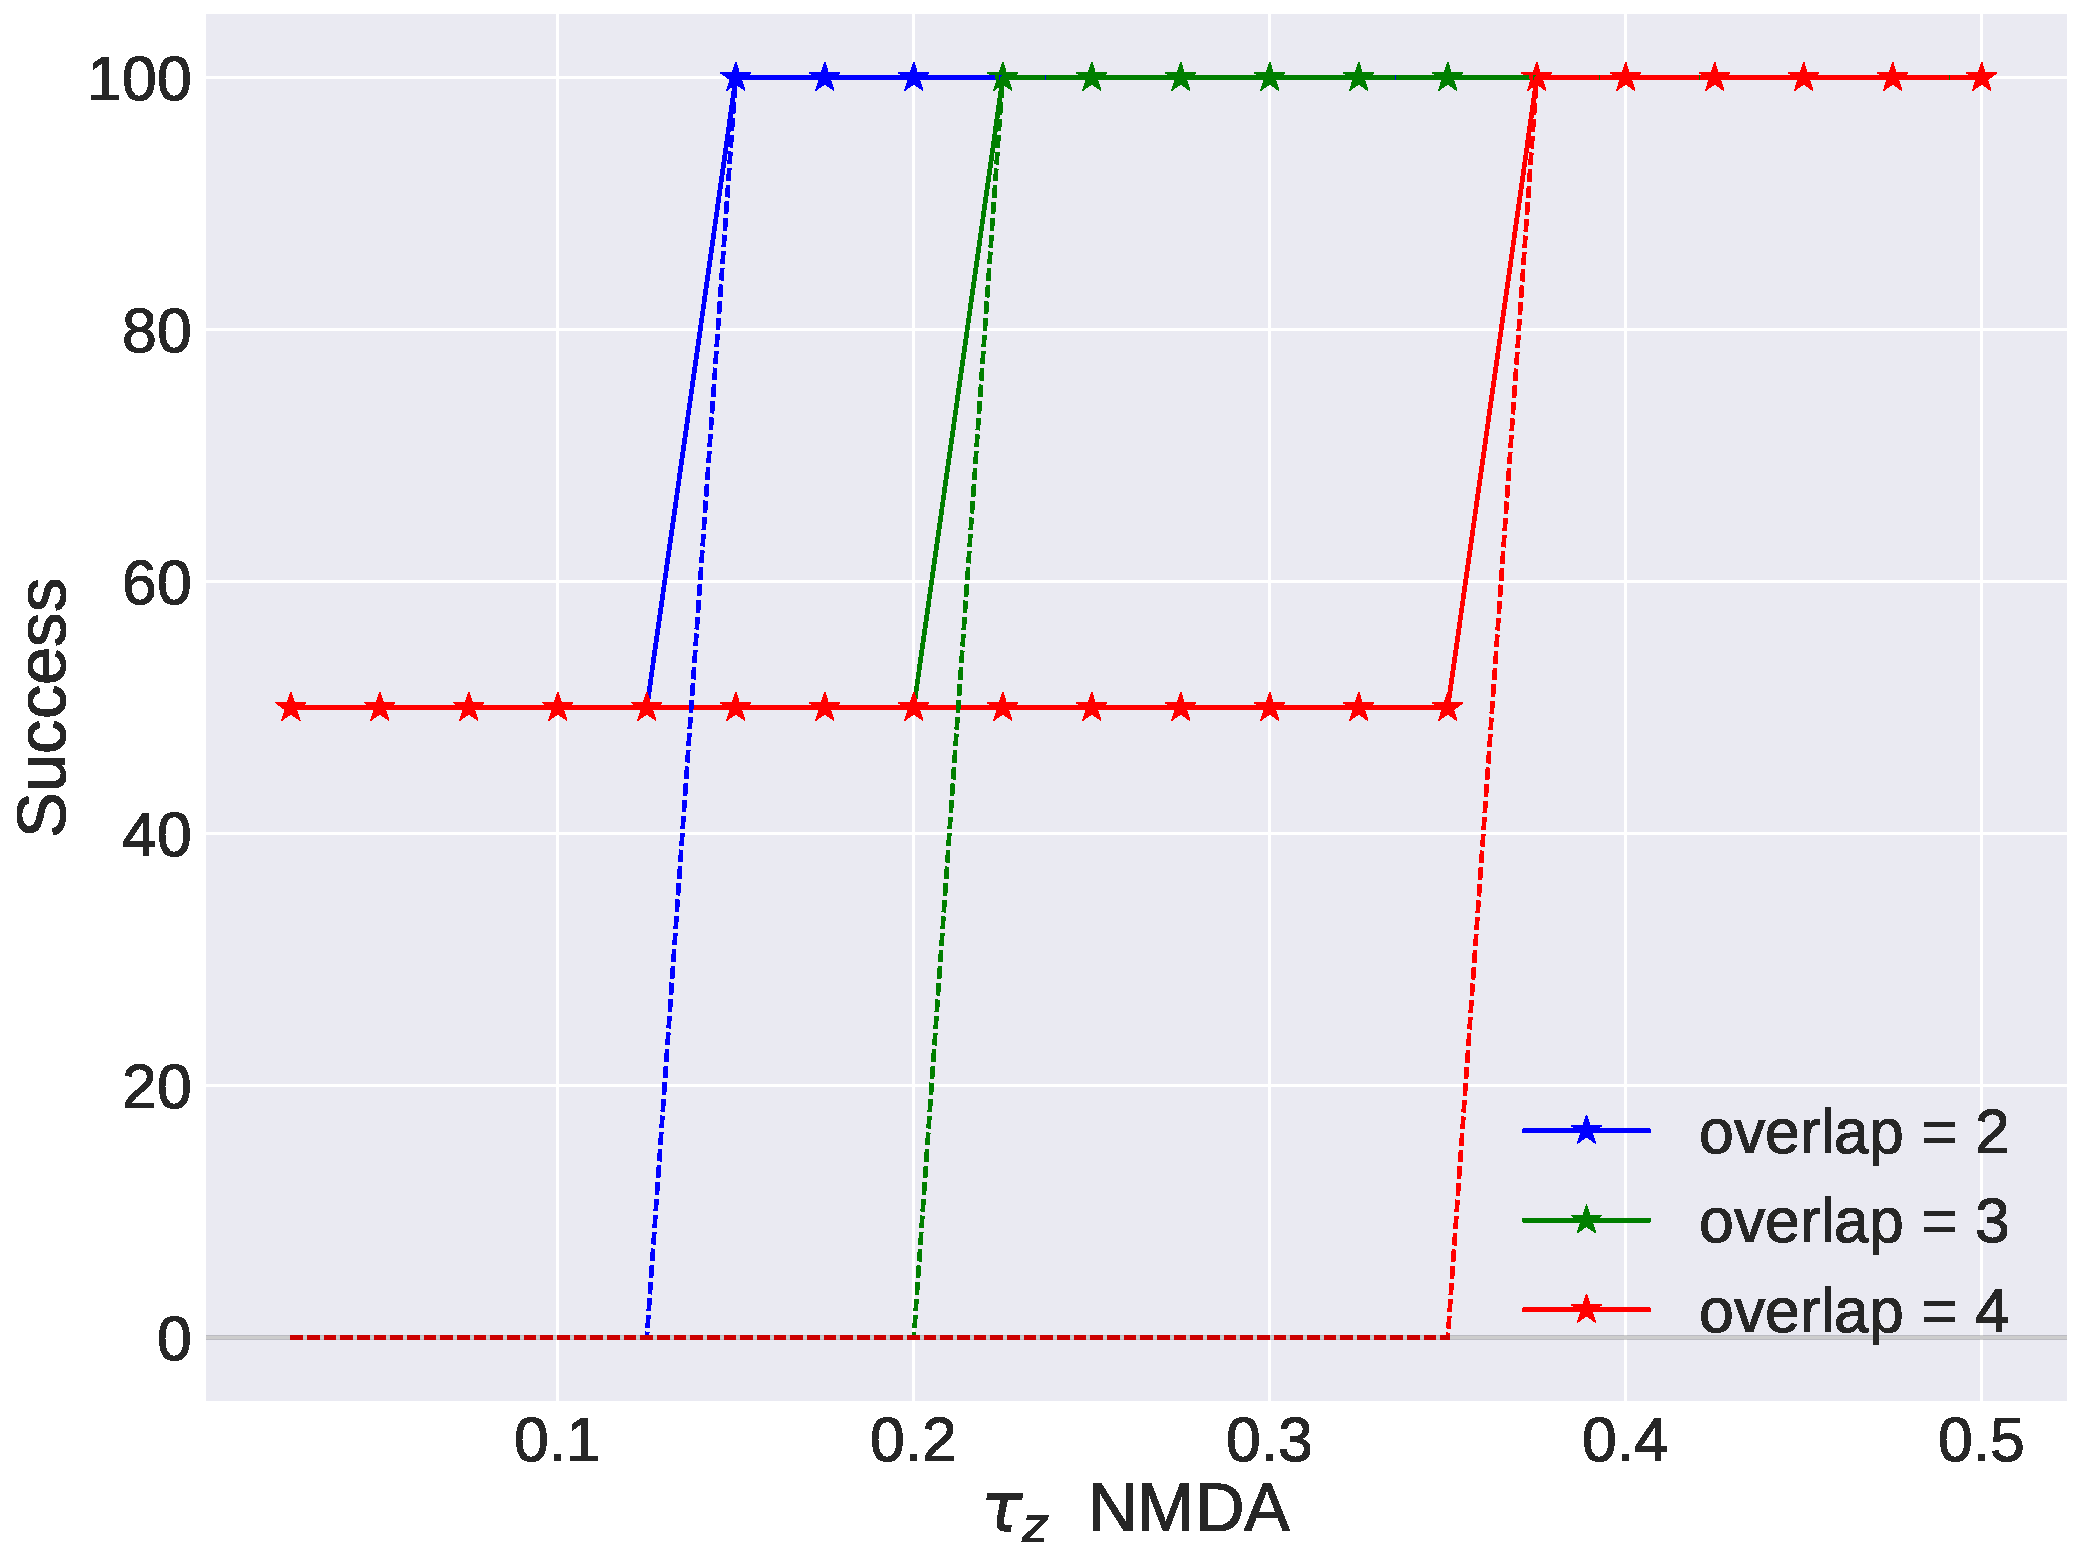
\includegraphics[scale=0.20]{capacity_tau_z.pdf}
\end{center}
}


%%%%%%%%%%%%%%%%%%%%%%%%%%%%%%%%%%%%%%%%%%%%%%%%%%%%%%%%%%%%%%%%%%%%%%%%%%%%%%%
\headerbox{Overload}{name=extension, column=2, span=1, below=chains}{
%%%%%%%%%%%%%%%%%%%%%%%%%%%%%%%%%%%%%%%%%%%%%%%%%%%%%%%%%%%%%%%%%%%%%%%%%%%%%%%

Here we calculate whether our system is able to correctly process the sequence with different degrees of overload for different values of the parameter $\tau_z $ NMDA.
\begin{center}
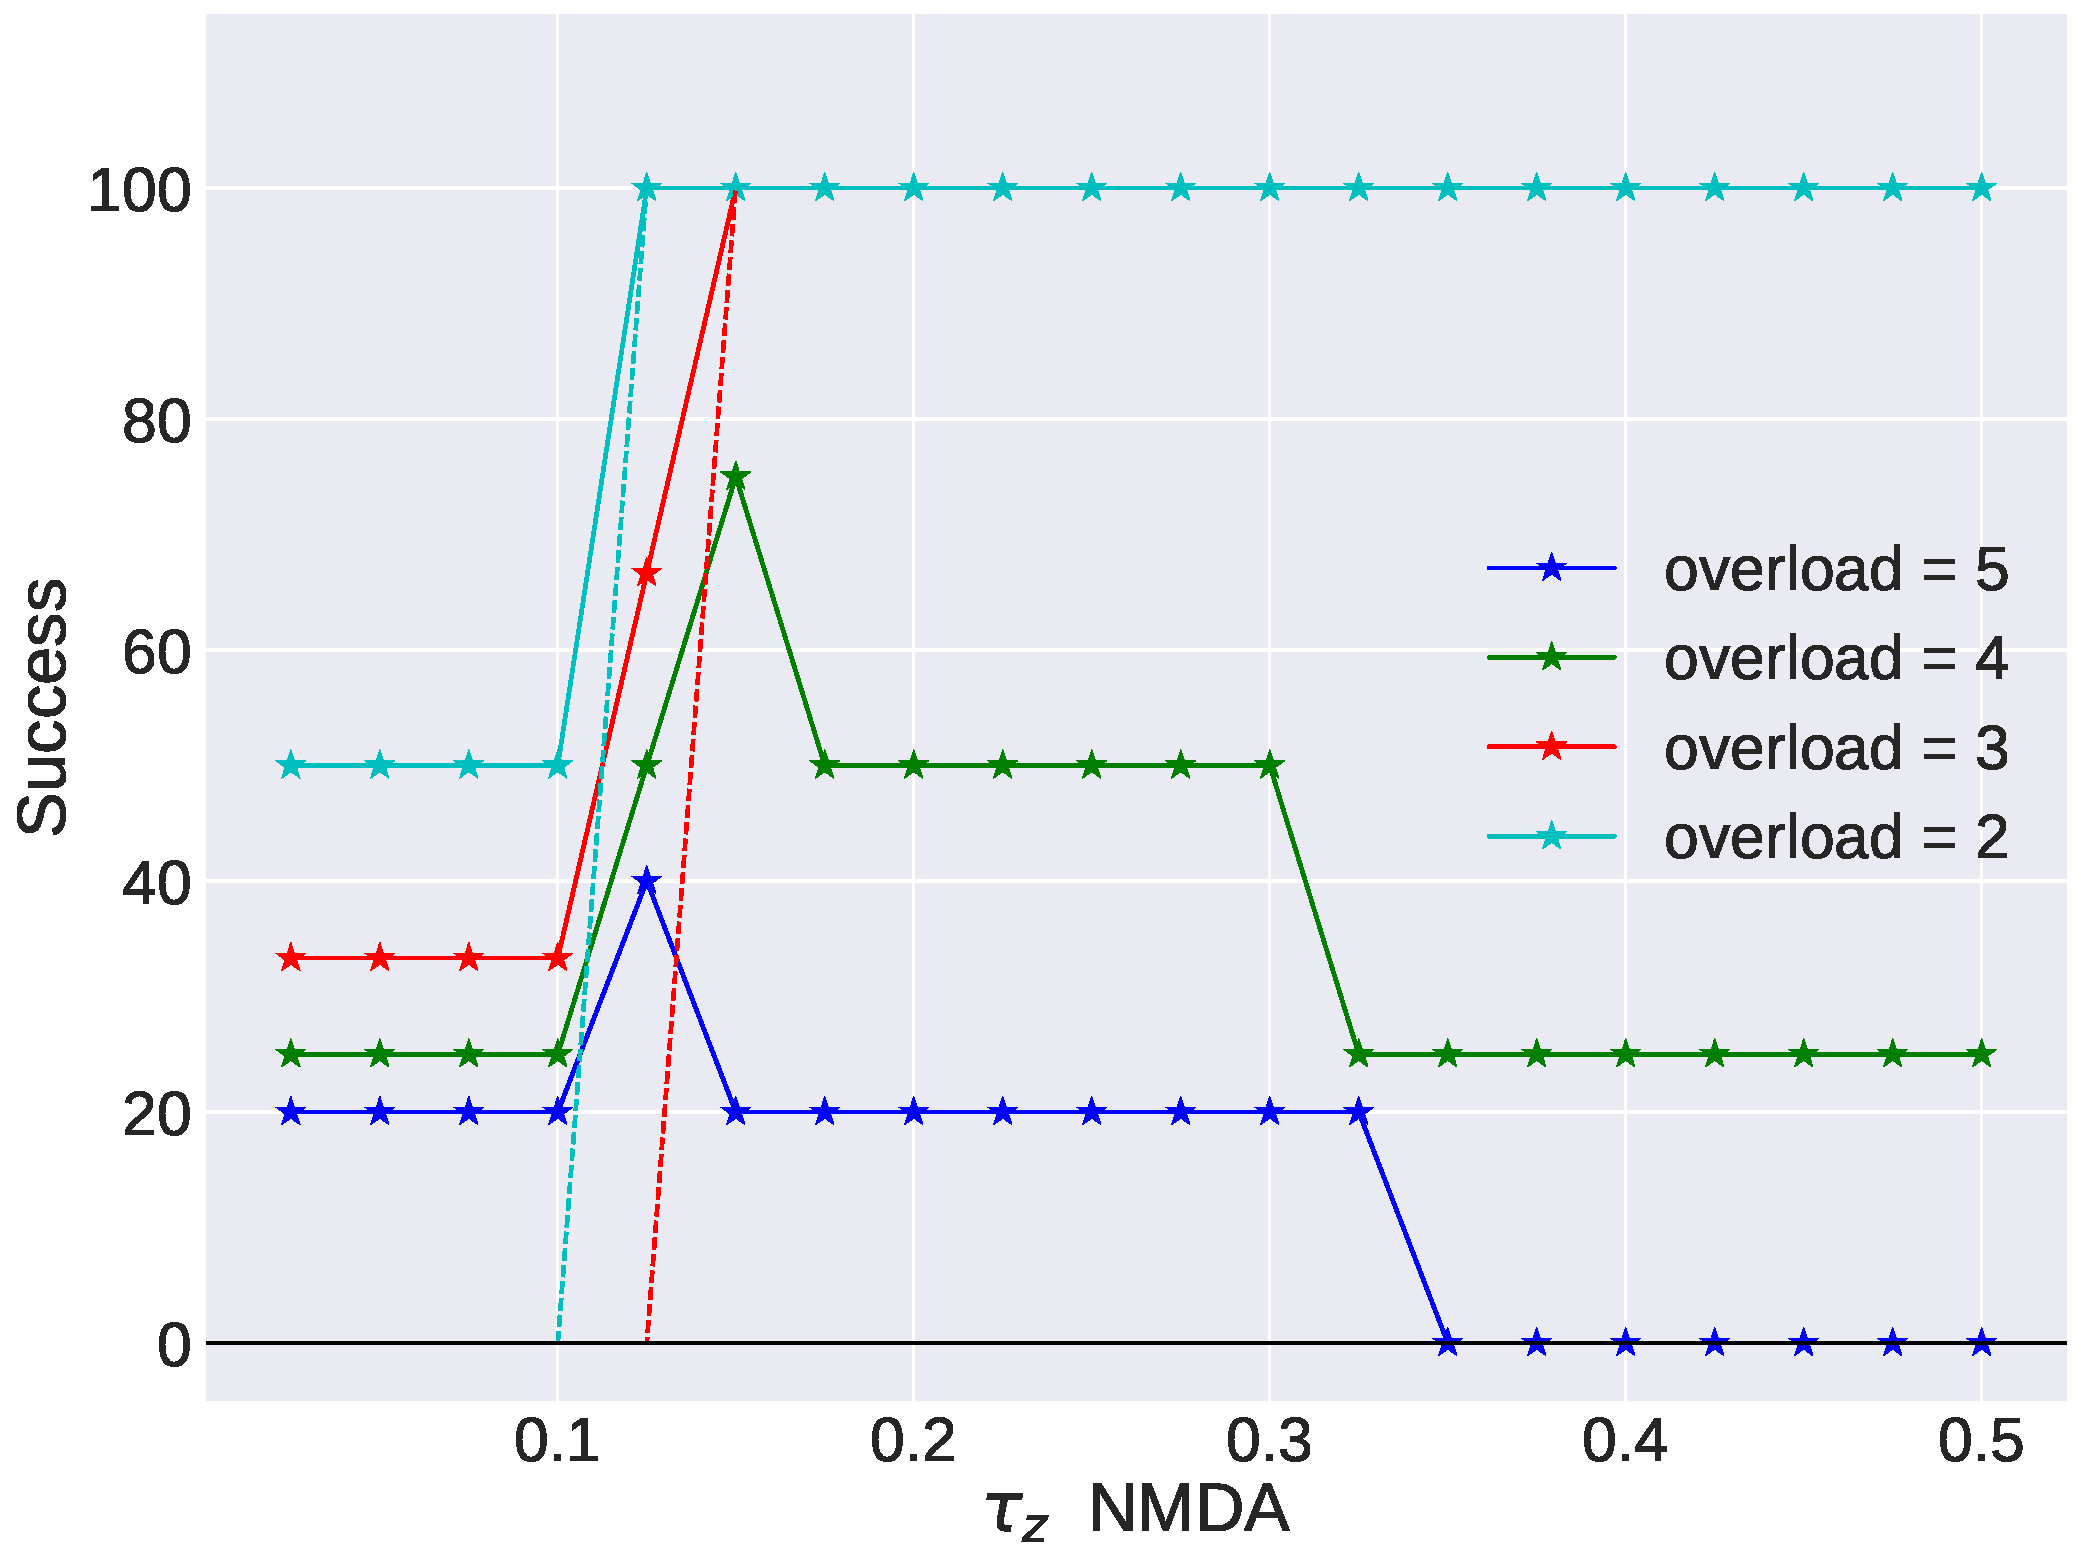
\includegraphics[scale=0.20]{capacity_tau_z_overload.pdf}
\end{center}
}


%%%%%%%%%%%%%%%%%%%%%%%%%%%%%%%%%%%%%%%%%%%%%%%%%%%%%%%%%%%%%%%%%%%%%%%%%%%%%%%
\headerbox{Funding}{name=funding,column=1,span=2,above=bottom}{
%%%%%%%%%%%%%%%%%%%%%%%%%%%%%%%%%%%%%%%%%%%%%%%%%%%%%%%%%%%%%%%%%%%%%%%%%%%%%%%
\begin{multicols}{2} 
 
 \smaller 
  \hspace{1em} This work was supported by the Erasmus Mundus Joint Doctoral Program Eurospin. 
  
 
\begin{center}

\includegraphics[height=6em]{logo_em.png}
\end{center}

\end{multicols}

}




\end{poster}%
\end{document}
